\chapter{Airborne Thermal Hyperspectral Data Properties}
\label{chap:Data}

This chapter provides insights into technical parameters of Thermal Airborne Spectrographic Imager (TASI) and processing chain of image data acquired by this sensor. Knowledge of the instrument parameters and processing chain gives important overview of the image data properties and their components. The result of the processing chain described in this chapter is georeferenced image data containing land-leaving radiance. Such an image data form an input for further processing. Let us note that this chapter omits naming physical quantities dependent on wavelength as ``spectral'' for the sake of clarity. However, all quantities remain wavelength dependent.

\section{Instrument Technical Specifications}

The TASI sensor is developed by Itres Ltd. (Calgary, Canada) and is one of the very few commercially available pushbroom hyperspectral TIR sensors equipped with mercury cadmium telluride array. Each of its 600 across-track imaging pixels contains 32 bands all of which are in the TIR region. Bands are situated in the 8 to $\SI{11.5}{\micro\meter}$ region and have a $\mathrm{FWHM} \approx \SI{0.11}{\micro\meter}$ with $\mathrm{NE\Delta T} \approx 0.1\,\mathrm{K}$. The response functions of the TASI sensor are described by the Gaussian functions as depicted in Figure \ref{fig:ResponseFunctionsChap2}. 

The shape of response functions implies that any quantity observed by TASI sensor is of finite spectral-bandwidth. Quantities needs to be transformed to band-effective quantities in order to relate them with certain wavelength. The band-effective quantities are obtained by using weighted average:
%Thus quantities measured by sensor are transformed to band-effective quantities using weighted average:
\begin{equation}
	X_i = \frac{\int_{\lambda_1}^{\lambda_2} r_i(\lambda) X(\lambda) \,\mathrm{d}\lambda}{\int_{\lambda_1}^{\lambda_2} r_i(\lambda)\,\mathrm{d}\lambda},
	\label{eq:weightedAverage}
\end{equation}
where $r_i(\lambda)$ is response function of band $i$, $\lambda_1$ and $\lambda_2$ are lower and upper boundaries of band $i$ and $X$ can be substituted by any quantity. In Figure \ref{fig:QuartzByTASIChap2} is illustrated radiance of quartz (solid line) and band-effective values of radiance measured by the TASI sensor (red dots). Sensor of this type is available at Global Change Research Institute CAS (Brno, Czech Republic) and it is a part of Flying Laboratory of Imaging Systems (FLIS) \cite{HF14}.

\begin{figure}[thb]
	\centering
	\vspace{1em}
	\begin{subfigure}[t]{.5\linewidth}
		\centering
		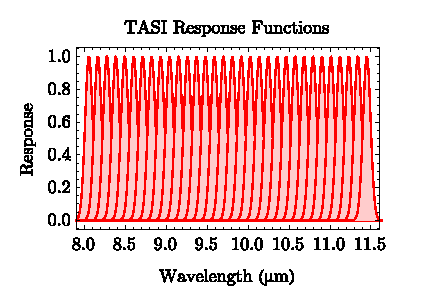
\includegraphics[scale=1]{pics/Chapter_02/TASIResponseFunctions.eps}
		\caption{Response functions of TASI sensor}
		\label{fig:ResponseFunctionsChap2}
	\end{subfigure}
	\hspace{2em}
	\begin{subfigure}[t]{.4\linewidth}
		\centering
		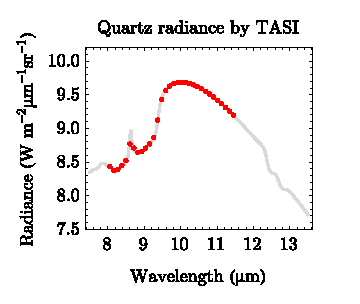
\includegraphics[scale=1]{pics/Chapter_02/QuartzByTASI.eps}
		\caption{Radiance of quartz at 300 K measured by TASI sensor}		
		\label{fig:QuartzByTASIChap2}
	\end{subfigure}
	\vspace{1.5 em}
	\caption{TASI response functions.}
\end{figure}

\section{Image Data Pre-processing}

The main objective of image data pre-processing is transformation of acquired raw image data into the georeferenced radiance at-surface level. It is accomplished by three major steps: radiometric calibration, atmospheric corrections and geometric pre-processing. Radiometric calibration converts digital numbers (DN) into values of radiance at-sensor level. Atmospheric corrections compensates the influence of intervening atmosphere and produces land-leaving radiance. Finally, the geometric pre-processing compensates for image data distortions caused by aircraft movement and register image data into coordinate system.

Supportive field measurements of thermal radiance, temperature, emissivity and atmospheric parameters offers valuable data for calibration and validation purposes. Especially in cases of airborne image data for scientific purposes the high quality is strongly demanding. Thus it is necessary to perform supportive measurements in order to achieve precise results and determine the data quality.

It is important to emphasize, that currently does not exist any definitive standard pre-processing chain. It is caused mainly by huge number of sensors with various technical parameters and their different applications. Sensors usually have tailored pre-processing chains, which is the case of TASI sensor as well. Certain parts of processing chain are maintained by commercial tools. However, there are still parts of processing chain, which needs to be done by in-house tools. In Figure \ref{fig:ProcessingChain} is illustrated processing chain used in Global Change Research Institute CAS (Brno, Czech Republic) to pre-process image data acquired by TASI sensor. Individual parts of the diagram will be discussed in the following text. The radiometric calibration and atmospheric corrections are demonstrated on example of quartz radiance at \SI{300}{\kelvin} as depicted in Figure \ref{fig:RadAtmCorOfQuartz}.

\begin{figure}[thb]
	\centering
	\vspace{0.7 em}
	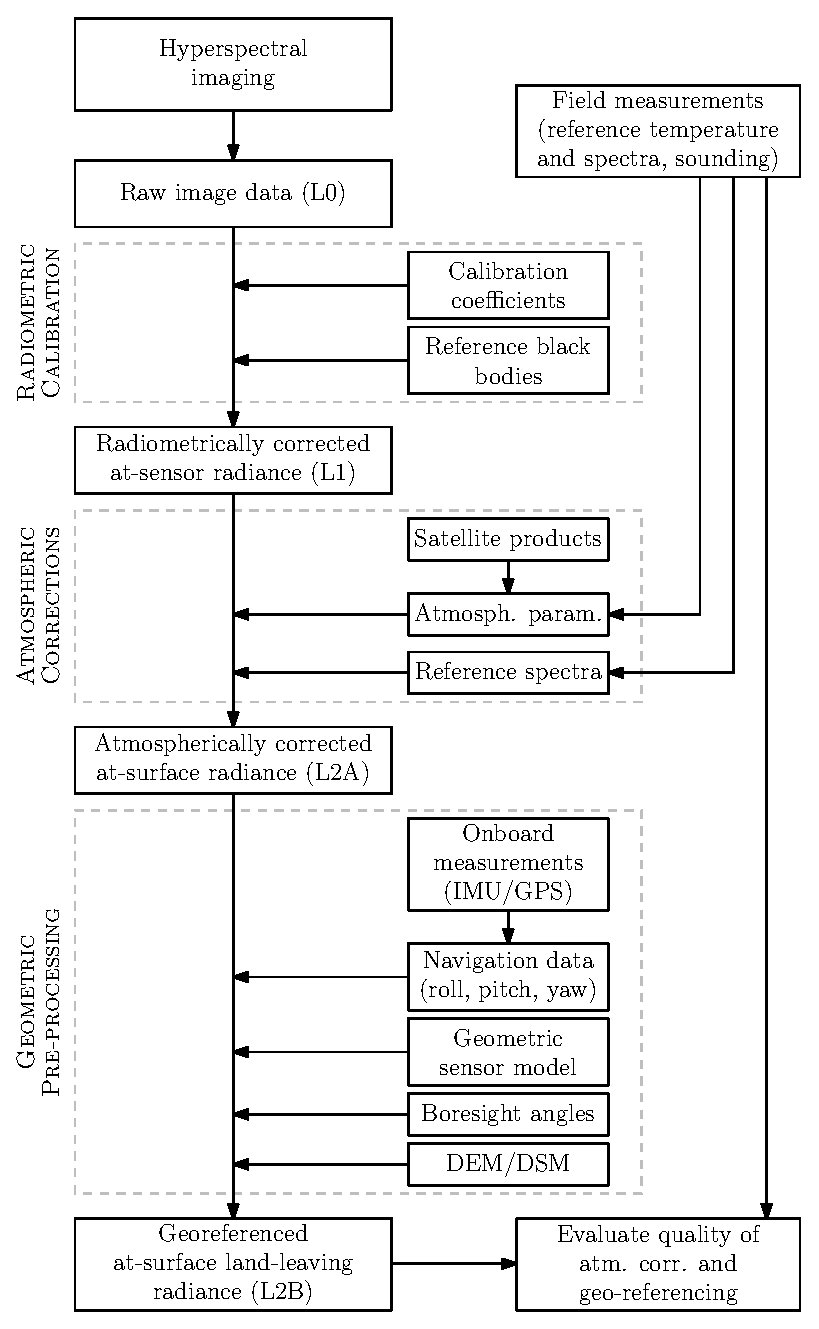
\includegraphics[scale=1]{pics/Chapter_02/Fig_2_3.eps}
	\label{fig:ProcessingChain}
	\vspace{2 em}
	\caption{Processing chain applied to image data acquired by TASI sensor.}
	\label{fig:ProcessingChain}
	\vspace{0.7 em}
\end{figure}

% show how are data modified by using different corrections -> three plots

\subsection*{Radiometric Calibration}

Thermal radiation incident upon the sensor array originates from many additive components (e.g. observed scene, instrument enclosure, intervening atmosphere and others). Incident thermal radiation produces electrical signal, which is proportional to radiant intensity. Electrical signal is then amplified and converted into voltage and subsequently into DN values (as depicted in Figure \ref{fig:RadAtmCorOfQuartz}a). Radiometric calibration consists of separating signal from viewed scene and converting it into physical units of radiance. Atmosphere influence is not accounted in this process and thus after radiometric calibration one gets radiance at-sensor level (as depicted in Figure \ref{fig:RadAtmCorOfQuartz}b).

The relationship between DN and at-sensor radiance $L_\mathrm{m}$ is following:
$$ \mathrm{DN} = a + b L_\mathrm{m}, $$
where $a$ and $b$ are calibration coefficients. The calibration coefficient $a$, also known as offset, represents radiation originating from instrument enclosure, sensor dark current and electronic offset. The calibration coefficient $b$, also called gain, determines sensor radiant sensitivity. Calibration coefficients are determined by imaging a set of reference black bodies of known temperature and emissivity. In this context, the term black body is ment to be a surface with emissivity very close to unity. These coefficients are usually determined applying one of two methods: 1) imaging two black bodies at different temperature directly before imaging, or 2) combining black body image data from laboratory and black body image data acquired before imaging.

In the first case are usually used two black bodies of different temperatures. Temperatures of these black bodies enclose temperatures expected to occur in the scene. Let us consider the radiance of cold black body $L(T_\mathrm{C})$ and the radiance of hot blackbody $L(T_\mathrm{H})$. The calibration coefficients can be obtained from:
\begin{eqnarray*}
	a &=& \frac{\mathrm{DN}_\mathrm{H} L(T_\mathrm{C}) - \mathrm{DN}_\mathrm{C} L(T_\mathrm{H}) }{ L(T_\mathrm{C}) - L(T_\mathrm{H}) } \\
	b &=& \frac{\mathrm{DN}_\mathrm{C} - \mathrm{DN}_\mathrm{H}}{ L(T_\mathrm{C}) - L(T_\mathrm{H}) },
\end{eqnarray*}
where $\mathrm{DN}_\mathrm{C}$ and $\mathrm{DN}_\mathrm{H}$ are digital numbers measured by sensor viewing cold black body and hot black body respectively. This procedure is commonly used in case of other instruments for measuring thermal radiation, such as $\mathrm{\mu}$FTIR \cite{HK96}.

The determination of calibration coefficients in the second case assumes that gain calibration coefficient $b$ does not change under different conditions. Thus, it is sufficient to perform series of black body measurements at different temperatures in order to determine gain calibration coefficient $b$. These measurements can be performed in the laboratory once per season. However, offset calibration coefficient $a$ does not remain stable and changes under different conditions. Hence, it is necessary to image a black body at known temperature directly before acquisition to account for variability of this coefficient.

%The determination of calibration coefficients in the second case is based on the assumption of invariant gain calibration coefficient $b$ and variable offset calibration coefficient $a$ in different conditions. This implies that gain calibration coefficient $b$ is determined in laboratory by imaging reference black bodies of different temperatures and offset calibration coefficient $a$ is determined by imaging reference black body of known temperature before acquisition of data from scene.

Again, it is important to emphasize that all quantities and both calibration coefficients are wavelength dependent. Spectral calibrations are part of the radiometric calibrations. In the laboratory are determined band centers of every pixel using laser at different wavelengths. Determined positions does not change over time significantly. However, the spectral shift occurs under different conditions and thus it needs to be determined for every scene. Spectral shift estimation is usually based on the spectral features of the atmosphere or certain materials.
% TODO: upresnit jednou vetou odhad spectral shiftu

In case of TASI sensor are used commercial softwares delivered by Itres company (Calgary, Canada). SparCal software \cite{software:SparCal} is used to determine all parameters necessary for radiometric calibrations from laboratory measurements. RCX software \cite{software:RCX} is used for additional  estimation of calibration parameters and for processing raw image data. Both softwares are tailored for the TASI sensor. The resulting image data are made of radiance at-sensor level $L_\mathrm{m}$.

\subsection*{Atmospheric Corrections}

Radiometric calibrations deliver image data containing radiation from the surface, attenuated by atmosphere, plus radiation from the atmosphere along the line of sight. Thus the measured radiance at-sensor level ($L_\mathrm{m}$) consists mainly of radiance emitted from the land surface, downwelling atmospheric radiance reflected by the surface ($L^\downarrow_\mathrm{atm}$) and the atmospheric upwelling radiance ($L^\uparrow_\mathrm{atm}$). The sum of all these components is expressed by a radiative transfer equation (RTE) as follows:
\begin{equation} 
\label{eq:RTE}
L_\mathrm{m} = \tau \varepsilon B(T_\mathrm{s}) + \tau (1 - \varepsilon) L^\downarrow_\mathrm{atm} + L^\uparrow_\mathrm{atm},
\end{equation}
where $B(T_\mathrm{s})$ is radiance of the surface at temperature $T_\mathrm{s}$ according to the Planck's law, $\varepsilon$ is the surface's emissivity and $\tau$ is atmospheric transmittance. It is important to emphasize that all elements in the equation are wavelength dependent but notation for this is omitted for the sake of clarity. Since sensors are of finite bandwidth, quantities in (\ref{eq:RTE}) are replaced by band-effective equivalents according to the (\ref{eq:weightedAverage}). Moreover, RTE can be used under the assumption of cloud-free atmosphere under local thermodynamic equilibrium. The meaning of the RTE is illustrated in the Figure \ref{fig:FigRTE}, where $\rho$ is reflectivity. Kirchhoff's law of thermal radiation implies that reflectivity $\rho$ can be rewritten as $(1 - \varepsilon)$ for opaque materials.

\begin{figure}[htbp]
	\centering
	\vspace{1em}
	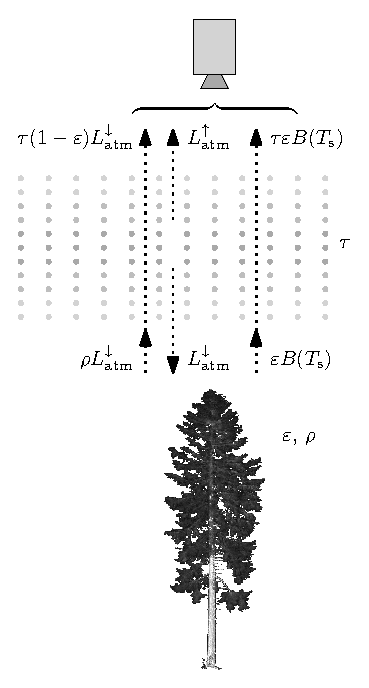
\includegraphics{pics/Chapter_02/Fig_3_2.eps}
	\vspace{1.5 em}
	\caption{The radiance incident to the sensor in the thermal region originates mainly from three sources: 1) radiance $\tau\varepsilon B(T_s)$ emitted by object; 2) reflected downwelling atmospheric radiance $\tau(1-\varepsilon)L_\mathrm{atm}^\downarrow$; 3) upwelling atmospheric radiance $L_{atm}^\uparrow$ emitted by atmosphere itself.}
	\label{fig:FigRTE}
\end{figure}

\newpage
The goal of the atmospheric corrections is to determine atmospheric transmittance, downwelling and upwelling atmospheric radiance and compensate for them. The quantification of these quantities are usually based on radiative transfer models of the atmosphere. For this purpose is usually used MODerate resolution atmospheric TRANsmission (MODTRAN) model \cite{BG06}. MODTRAN simulates atmospheric parameters such as atmospheric transmittance, downwelling and upwelling atmospheric radiance based on input parameters such as vertical profiles of water vapour content and temperature, CO$_2$ concentration, the choice of model atmosphere (if measured profiles are not available) and many others. In general, input parameters can be obtained in two ways: 1) by \textit{in-situ} measurements; 2) by satellite-based products.

The most common \textit{in-situ} measurement is radio sounding. Radiosonde is launched during the overflight and it is used to measure vertical temperature and water vapour profile of the atmosphere. Other \textit{in-situ} instruments can be used as well, for example sun-photometer for obtaining water vapor content or different radiometers for measuring sky or surface radiance. Other source of water vapour and temperature profile is satellite-based products acquired close to the time of aircraft overflight. The most common is MOD07\_L2 product \cite{B11} generated by Moderate Resolution Imaging Spectroradiometer (MODIS) instrument. Illustration of the transmittance, downwelling and upwelling atmospheric radiance generated by MODTRAN using MOD07\_L2 products as input are depicted in Figure \ref{fig:AtmParams}.

\begin{figure}[htb]
	\centering
	\vspace{1em}
	\begin{subfigure}[t]{.3\linewidth}
		\centering
		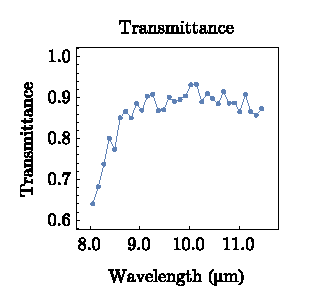
\includegraphics[scale=1]{pics/Chapter_02/Transmittance.eps}
		\vspace{-0.4cm}
		%\caption{Atmospheric transmittance}
		\caption{}
	\end{subfigure}
	\hspace{1em}
	\begin{subfigure}[t]{.3\linewidth}
		\centering
		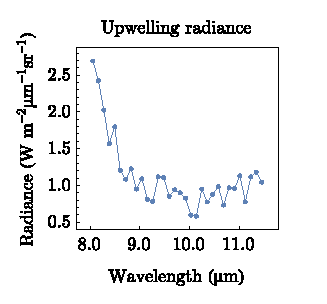
\includegraphics[scale=1]{pics/Chapter_02/Upwelling.eps}
		\vspace{-0.4cm}
		%\caption{Upwelling atmospheric radiance}
		\caption{}
	\end{subfigure}
	\hspace{1em}
	\begin{subfigure}[t]{.3\linewidth}
		\centering
		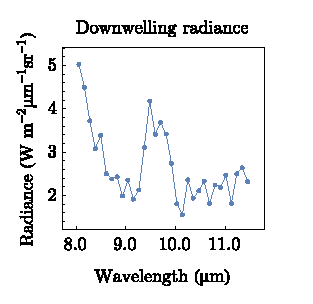
\includegraphics[scale=1]{pics/Chapter_02/Downwelling.eps}
		\vspace{-0.4cm}
		%\caption{Downwelling atmospheric radiance}
		\caption{}
	\end{subfigure}
	\vspace{1.5 em}
	\caption{Example of atmospheric parameters used for atmospheric correction of TASI image data acquired at altitude of \SI{2000}{\meter} during summer season.}
	\label{fig:AtmParams}
\end{figure}

In case of thermal hyperspectral images, various algorithms for estimating atmospheric effects based just on the image data itself were developed. Usually it is applied to one of the following: In-Scene Atmospheric Corrections (ISAC) introduced by Young et al. \cite{Y02} and Autonomous Atmospheric Compensation (AAC) introduced by Gu et al. \cite{GG00}. The advantage of using one of these algorithms is that no supporting data are necessary. The drawback of these methods remains in estimation of just atmospheric transmittance and upwelling atmospheric radiance.

Once all the atmospheric parameters are determined, it remains to compensate for them. Compensating for atmospheric transmittance and upwelling atmospheric radiance lead to land-leaving radiance:
\begin{equation}
\label{eq:landleavingRadiance}
L_\mathrm{LL} = \varepsilon B(T_\mathrm{s}) + (1 - \varepsilon) L^\downarrow_\mathrm{atm}.
\end{equation}
The example of land-leaving radiance is shown in Figure \ref{fig:RadAtmCorOfQuartz}c. The downwelling atmospheric radiance is not possible to separate without knowledge of emissivity. Hence, image data after atmospheric corrections are made of land-leaving radiance $L_\mathrm{LL}$. Compensation for downwelling atmospheric radiance is part of the temperature and emissivity separation described in Chapter \ref{chap:TES}.

Atmospheric corrections for TASI sensor, as part of processing chain, are not performed by commercial products. However, there exists commercial tools that allows complex solution for atmospheric corrections. An example of such a tool is ATCOR \cite{RS02} which is based on look-up tables generated by MODTRAN and takes into account terrain topography and sensor parameters. It offers basic temperature and emissivity separation algorithms as well. Apart of mentioned solution, atmospheric corrections rely on extracting data from \textit{in-situ} measurements or satellite products, running radiative transfer models and applying derived atmospheric parameter on image data. Alternatively, algorithms for atmospheric parameters estimation from image data can be implemented. In both cases, atmospheric corrections involve creating in-house tools.

\begin{figure}[htb]
	\centering
	\vspace{1em}
	\begin{subfigure}[t]{.3\linewidth}
		\centering
		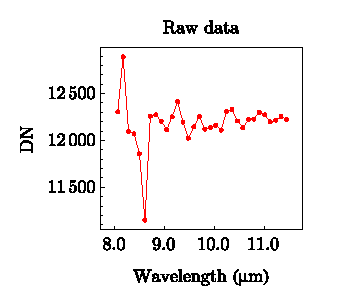
\includegraphics[scale=1]{pics/Chapter_02/calibration-1-DN.eps}
		\vspace{-0.4cm}
		%\caption{Raw image of quartz in DN values}
		\caption{}
	\end{subfigure}
	\hspace{1em}
	\begin{subfigure}[t]{.3\linewidth}
		\centering
		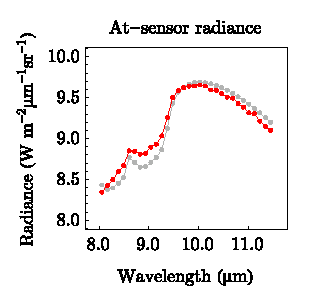
\includegraphics[scale=1]{pics/Chapter_02/calibration-2-Lm.eps}
		\vspace{-0.4cm}
		%\caption{At-sensor radiance of quartz}
		\caption{}
	\end{subfigure}
	\hspace{1em}
	\begin{subfigure}[t]{.3\linewidth}
		\centering
		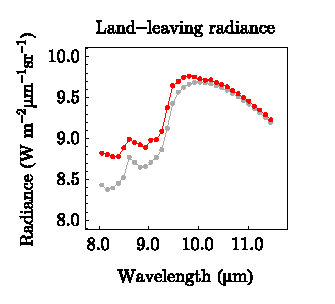
\includegraphics[scale=1]{pics/Chapter_02/calibration-3-Lll.eps}
		\vspace{-0.4cm}
		%\caption{Land-leaving radiance of quartz.}
		\caption{}
	\end{subfigure}
	\vspace{1.5 em}
	\caption{Example of data at various processing stages. Data simulates quartz at \SI{300}{\kelvin} as would be acquired by TASI sensor at altitude of \SI{2000}{\meter} under summer mid-latitude atmosphere. Case (a) shows raw data, case (b) shows data after radiometric calibration (in red) and case (c) shows data after corrections of atmospheric transmissivity and upwelling atmospheric radiance (in red). In cases (b) and (c) are shown pure quartz radiance in gray.}
	\label{fig:RadAtmCorOfQuartz}
\end{figure}

\subsection*{Geometric Pre-processing}

Acquired image data are distorted during its acquisition and geometric pre-processing is accounting for all factors causing these distortions. During geometric pre-processing are taken into account aircraft motion, terrain variations and geometric sensor model in order to register image data into reference frame.

Ancillary data about aircraft position and movement, terrain structure and geometric sensor model are necessary. Aircraft needs to be equipped with IMU/GNSS systems for recording aircraft position (longitude, latitude and altitude) and orientation (roll, pitch and heading angles). Terrain structure is obtained form Digital Surface Model (DSM) or Digital Elevation Model (DEM). These data are derived from aerial laser scanning or from stereo images. Aerial laser scanning can be performed either simultaneously with image data acquisition or separately. Other sources of DEM/DSM are national services or~satellite products (e.g. ASTER product AST14DEM). Geometric sensor model is usually delivered by sensor manufacturer.

The process applied on image data during geometric pre-processing is called geo-othoreferencing. It consists of two successive steps: direct image data geocoding and resampling. Direct image data geocoding consists of geometric corrections and orthogonalization of the image data. These are further resampled into regular grid of the reference frame with the desired coordinate system (e.g. Universal Transverse Mercator coordinate system). Image data are resampled into desired spatial resolution applying nearest neighbor, bilinear or cubic interpolation. For the scientific purposes is commonly used nearest neighbor interpolation since it preserves spectral information and does not combine spectra from surrounding pixels.

Geometric pre-processing of the image data acquired by TASI sensor are performed by GeoCor software \cite{software:GCSS} delivered by Itres company (Calgary, Canada). Importance of image data geometric pre-processing is illustrated in the Figure \ref{fig:Georeferencing}. 

\begin{figure}[thb]
	\centering
	\vspace{1em}
	\begin{subfigure}[t]{.38\linewidth}
		\centering
		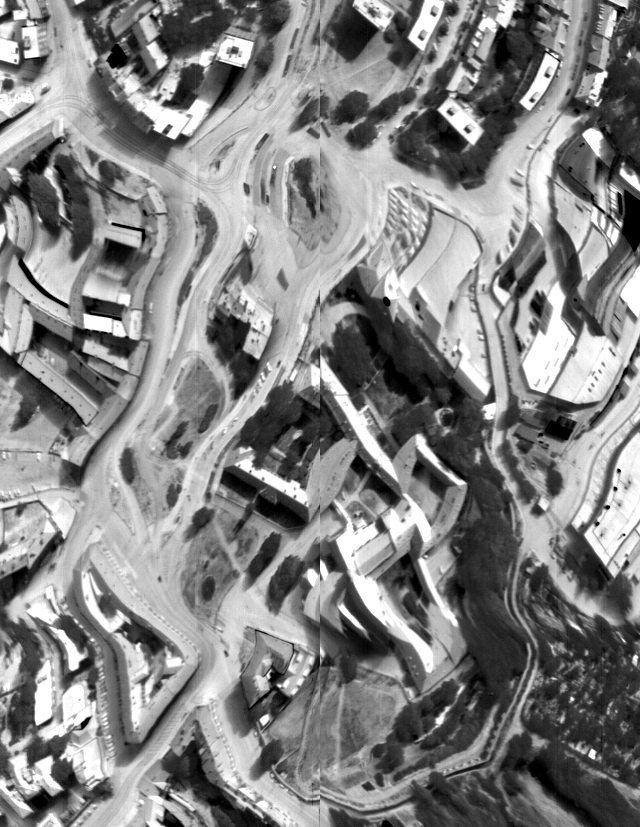
\includegraphics[scale=0.24]{pics/Chapter_02/TASIcalibrated.png}
		\caption{Distorted image data}
		\label{fig:ResponseFunctions}
	\end{subfigure}
	\hspace{2em}
	\begin{subfigure}[t]{.52\linewidth}
		\centering
		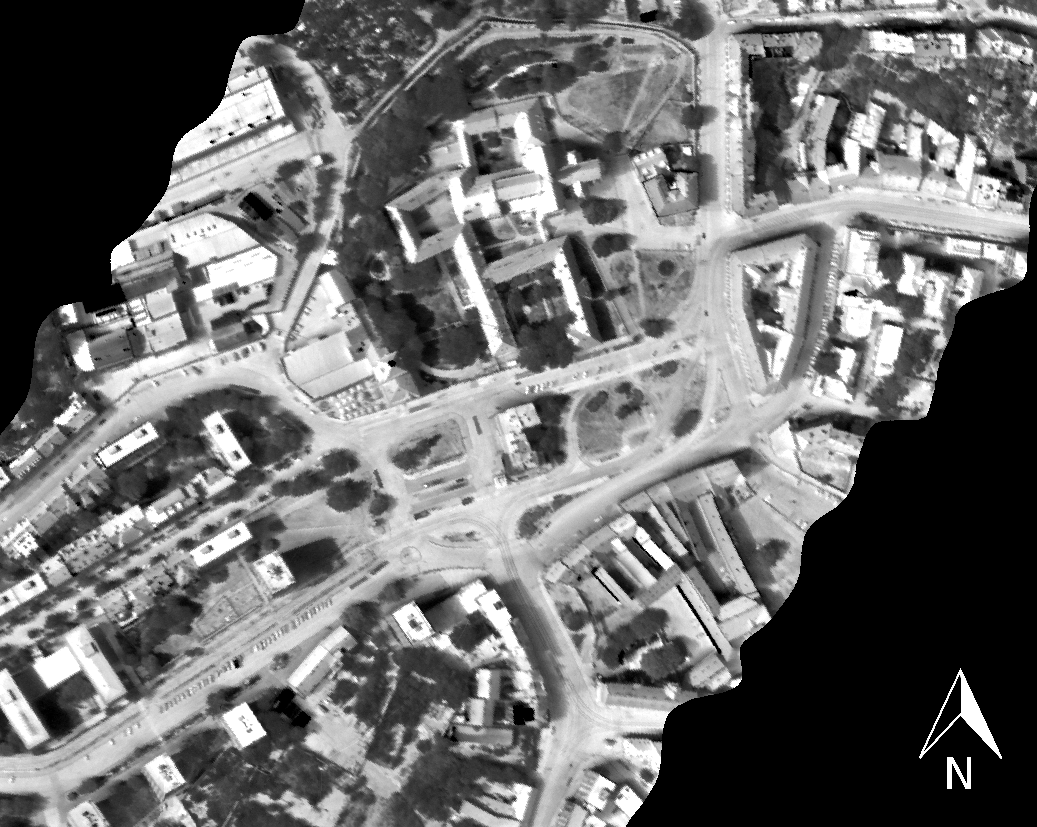
\includegraphics[scale=1]{pics/Chapter_02/TASIgeoreferencedcut.png}
		\caption{Georeferenced image data}		
		\label{fig:QuartzByTASI}
	\end{subfigure}
	\vspace{1.5 em}
	\caption{Illustration of land-leaving radiance image data before and after geometric pre-processing.}
	\label{fig:Georeferencing}
\end{figure}


